\begin{center}
 \begin{minipage}[b]{0.45\textwidth} 
\subsection*{General information}
Name: David Nikolaj Vinje 
Address: Islands brygge 56b 1tv
Zip nr. 2300 Koebenhavn S
number: 12345678
E-mail: david2300@hotmail.com
Country: Danmark
Date of birth: 11/06/1995
\newline \end{minipage}
 \hfill
\begin{minipage}[b]{3cm}
 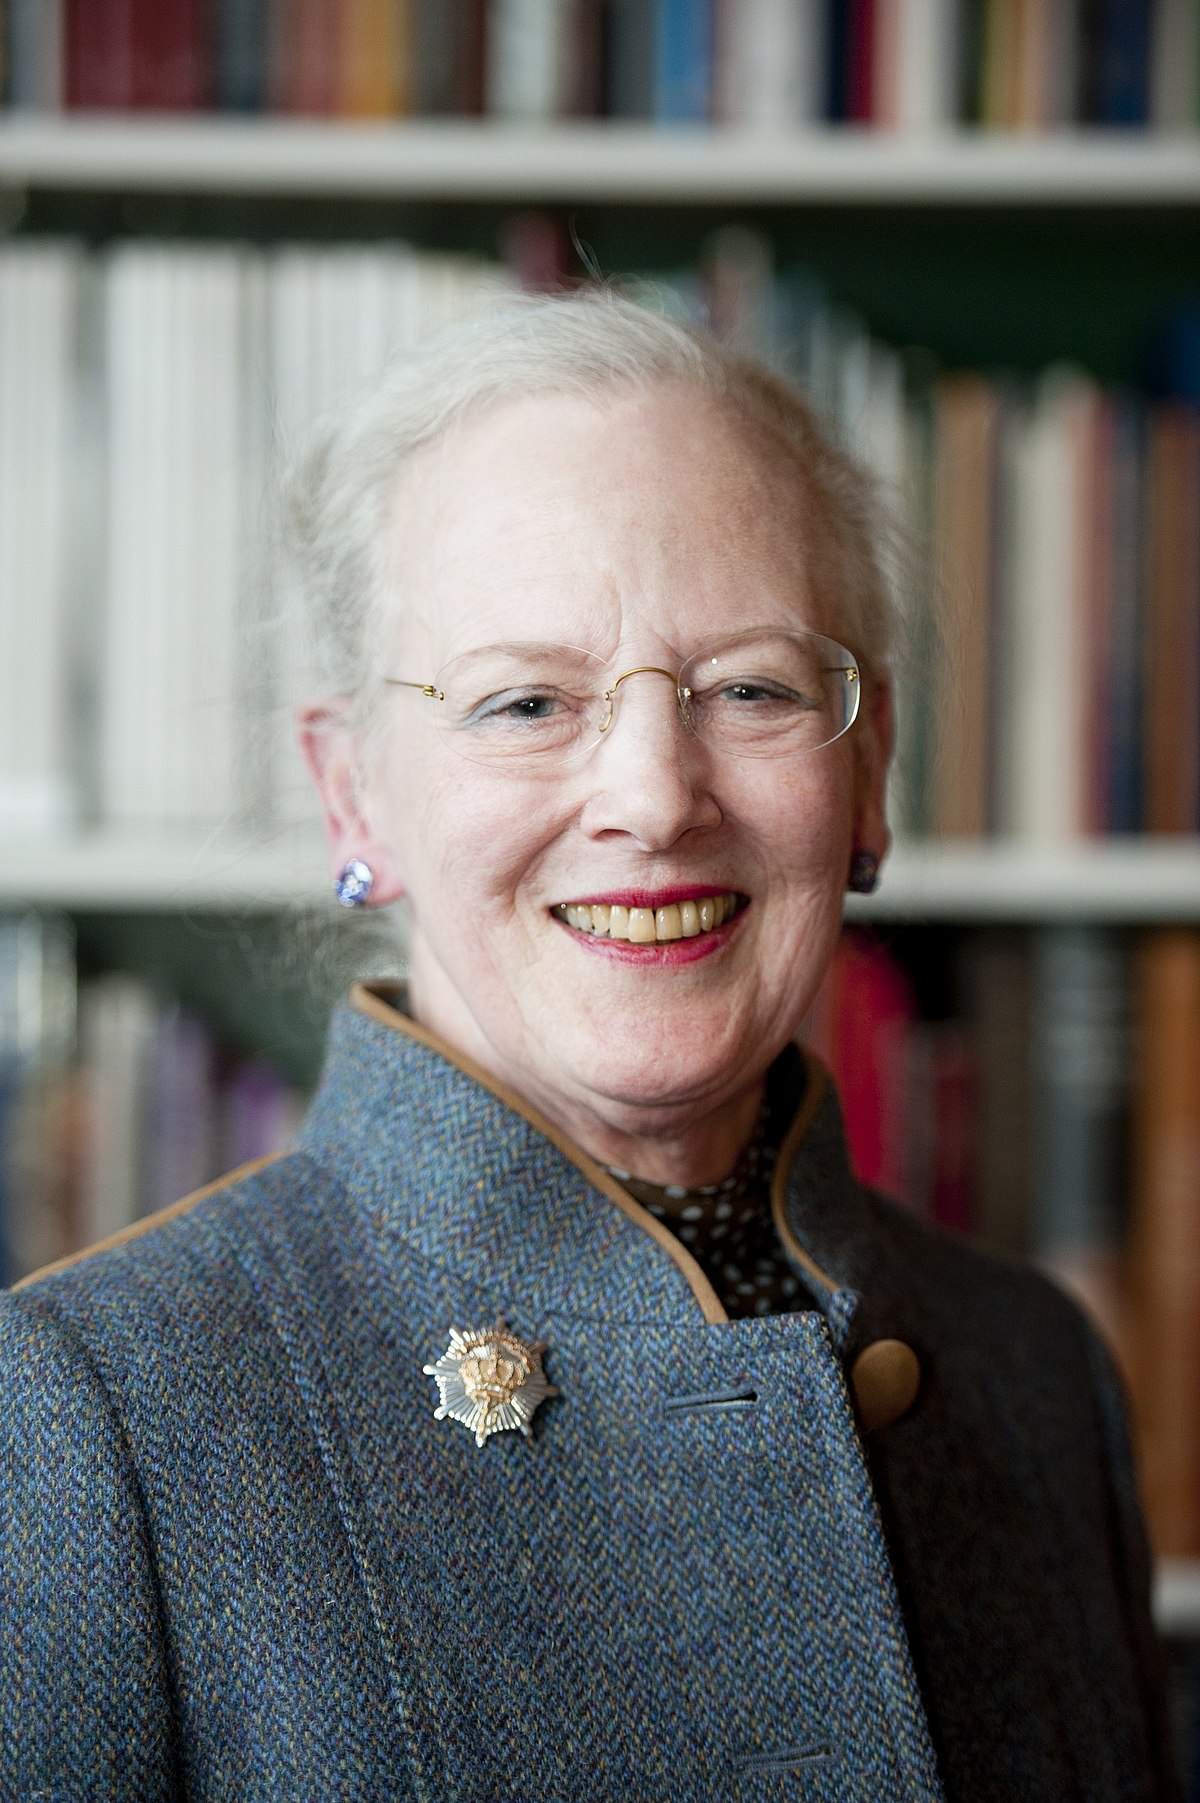
\includegraphics[height=4cm]{figures/1200px-Drottning_Margrethe_av_Danmark}
 \end{minipage}
 \end{center}

\section*{Workexperience}
\begin{itemize}
\item 2009-2011 Flaskedreng i Netto.
\item 2011-2013 .
\end{itemize}
\section*{Education}
\begin{itemize}
\item 2016-2019 AAU Batchelor i software.
\item 2013-2016 HTX-Hilleroed, Mat-Fys.
\end{itemize}

\section*{Free text}
Took a highschool diploma in Biotechnology and chemistry, where i ended with a grade of 10.7.
Took a highschool diploma in Biotechnology and chemistry: capable of doing PCR testing.
Highschool exam project was using c sharp (unity) to make a game.
Currently doing a bsc in engineering (software) at Aalborg university.
University focuses on teamwork, so i have lots of experience with larger groups.
Lots of skills in programming.
Large interest in electronics. Done multiple projects.
Capable of using machine learning using python. Also read a lot of statistics and probability theory to learn the theory behind it. Can use neural networks, to predict behavior.
Degree in computer science.

